\chapter{Automatic Differentiation}
All modern libraries for neural networks, i.e.~\href{https://www.tensorflow.org}{TensorFlow} and
\href{https://pytorch.org}{PyTorch} make heavy use of
\href{https://en.wikipedia.org/wiki/Automatic_differentiation}{automatic differentiation}.
\blue{Automatic differentiation} is a technique for computing the gradient of a function that does neither rely
on numeric approximation nor does it force us to compute symbolic derivatives manually.  In fact, the technique
is one of the major methodological breakthroughs in machine learning in particular and science and engineering
in general in recent years.  Although the idea was first published in 1964 by R.~E.~Wengert \cite{wengert:1964},
it has only been widely understood and accepted in recent years, cf.~Baydin et.~al.~\cite{baydin:2018}.

There are two modes of automatic differentiation:  \blue{Forward mode} and \blue{reverse mode}.  Forward
mode is quite inefficient when the number $n$ of input variables is big.  The reason is that forward mode needs
to traverse the \blue{computational graph} $n+1$ times (once to compute the values and $n$ times to compute the
partial derivatives), while reverse mode needs to traverse the computational graph just twice.  Hence for big
values of $n$ only reverse mode automatic differentiation is a viable option.  We proceed to define the crucial
notion of a computational graph. 

\begin{Definition}[Computational Graph] 
  A \blue{computational graph} \index{computational graph} is a list of \blue{computational nodes}.
  \index{computational node}  There are four types of computational nodes:
  \begin{enumerate}
  \item A \blue{variable node} is tuple of length 1 of the form   
        \\[0.2cm]
        \hspace*{1.3cm}
        $\langle x, \rangle$
        \\[0.2cm]
        where $x$ is a variable from the set of variables $\{x_1,\cdots,x_k\}$.
        This node represents the given input variable.
  \item A \blue{constant node} is a pair of the form
        \\[0.2cm]
        \hspace*{1.3cm}
        $\langle n, r\rangle$
        \\[0.2cm]
        where $n$ is the \blue{name} of the node and $r$ is a floating point number.  This node is interpreted
        as the assignment
        \\[0.2cm]
        \hspace*{1.3cm}
        $n \;\mathtt{:=}\; r$.
        \\[0.2cm]
        The name $n$ is a string that can be understood as the name of an auxiliary variable.
  \item A \blue{unary node} is a tuple of the form
        \\[0.2cm]
        \hspace*{1.3cm}
        $\langle n, f, a\rangle$
        \\[0.2cm]
        where, again, $n$ is the \blue{name} of the node that is used as an auxiliary variable. $f$ is an unary
        function symbol from a set of unary function.  In our examples $f$ will be a mwember of the set 
        \\[0.2cm]
        \hspace*{1.3cm}
        $\{ \mathrm{sqrt}, \exp, \ln, \sin, \cos, \arctan \}$
        \\[0.2cm]
        and $a$ is the name of another node occurring in the list.  This node is interpreted as the assignment
        \\[0.2cm]
        \hspace*{1.3cm}
        $n \;\mathtt{:=}\; f(a)$.        
  \item A \blue{binary node} is a tuple of the form
        \\[0.2cm]
        \hspace*{1.3cm}
        $\langle n, o, a_1, a_2\rangle$
        \\[0.2cm]
        where $n$ is the \blue{name} of the node, $o$ is a binary operator from the set
        \\[0.2cm]
        \hspace*{1.3cm}
        $\{ +, -, *, / \}$
        \\[0.2cm]
        and $a_1$ and $a_2$ are the names of computational nodes.
        
        This node is interpreted as the assignment
        \\[0.2cm]
        \hspace*{1.3cm}
        $n \;\mathtt{:=}\; a_1\; o\,\; a_2$.
        \\[0.2cm]
        As in the previous case, the name $n$ is a string that can be understood as the name of an auxiliary
        variable. 
        \eoxs
 \end{enumerate}
\end{Definition}

\begin{figure}[!ht]
\centering
\begin{minted}[ frame         = lines, 
                 framesep      = 0.3cm, 
                 firstnumber   = 1,
                 bgcolor       = sepia,
                 numbers       = left,
                 numbersep     = -0.2cm,
                 xleftmargin   = 0.8cm,
                 xrightmargin  = 0.8cm,
               ]{python3}
    CG = [ ('x1', ),
           ('x2', ),
           ('v1', '+',   'x1', 'x2'),
           ('v2', '-',   'x1', 'x2'),
           ('v3', 'sin', 'v1'),
           ('v4', 'cos', 'v2'),
           ('v5', '*',   'v3', 'v4'),
           ('v6', '*',   'v1', 'v2'),
           ('y',  '+',   'v5', 'v6')
         ]
\end{minted}
\vspace*{-0.3cm}
\caption{A Computational Graph for $\sin(x_1 + x_2) \cdot \cos(x_1 - x_2) + (x_1 + x_2) \cdot (x_1 - x_2)$.}
\label{fig:computational-graph}
\end{figure}
\example
Figure \ref{fig:computational-graph} shows a computational graph for the expression
\\[0.2cm]
\hspace*{1.3cm}
$\sin(x_1 + x_2) \cdot \cos(x_1 - x_2) + (x_1 + x_2) \cdot (x_1 - x_2)$.
\\[0.2cm]
This computational graph uses the input variables \texttt{x1} and \texttt{x2}.
Figure \ref{fig:cg.eps} shows a rendering of this computational graph. \eoxs

\begin{figure}[!ht]
\centering
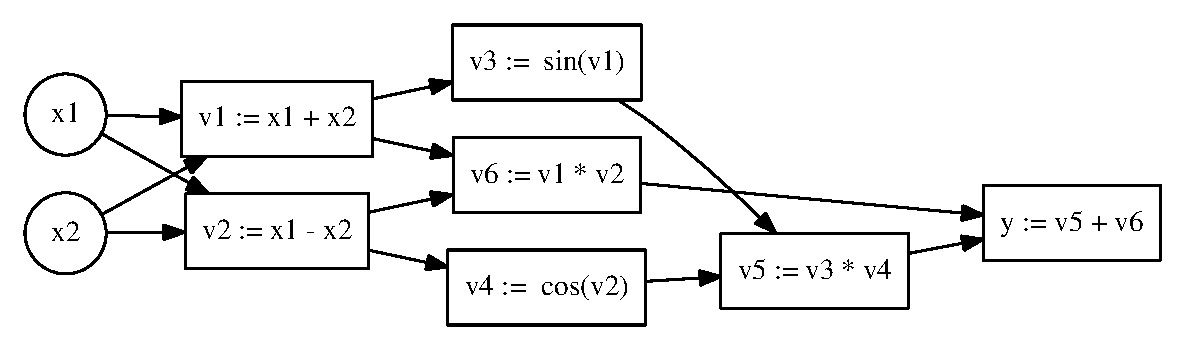
\epsfig{file=Figures/cg.eps,scale=0.8} \
\vspace*{-0.3cm}
\caption{Rendering of the computation graph shown in Figure \ref{fig:computational-graph}.}
\label{fig:cg.eps}
\end{figure}

\begin{Definition}[admissible]
A computational graph $G$ is \blue{admissible} \index{admissible, computational graph} if for every node of the form
\\[0.2cm]
\hspace*{1.3cm}
$\langle n, o, a_1, a_2\rangle$
\\[0.2cm]
that occurs in the list $G$ there are nodes labelled with $a_1$ and $a_2$ that occur in the list $G$ \underline{before} this node and for
every  node of the form
\\[0.2cm]
\hspace*{1.3cm}
$\langle n, f, a\rangle$
\\[0.2cm]
that occurs in the list $G$ there is a node labelled with $a$ that occurs in the list G \underline{before} this node.
If a computational graph is admissible, the nodes can be evaluated in the same order as they are listed in $G$.
\eoxs
\end{Definition}
\begin{figure}[!ht]
\centering
\begin{minted}[ frame         = lines, 
                 framesep      = 0.3cm, 
                 firstnumber   = 1,
                 bgcolor       = sepia,
                 numbers       = left,
                 numbersep     = -0.2cm,
                 xleftmargin   = 0.8cm,
                 xrightmargin  = 0.8cm,
               ]{python3}
    def eval_graph(CG, Values):
        for node in CG:
            match node:
                case (v, ):
                    pass
                case (v, r):
                    Values[v] = r
                case (v, '+', a1, a2):
                    Values[v] = Values[a1] + Values[a2]
                case (v, '-', a1, a2):
                    Values[v] = Values[a1] - Values[a2]
                case (v, '*', a1, a2):
                    Values[v] = Values[a1] * Values[a2]
                case (v, '/', a1, a2):
                    Values[v] = Values[a1] / Values[a2]
                case (v, 'sqrt', a):
                    Values[v] = math.sqrt(Values[a])            
                case (v, 'exp', a):
                    Values[v] = math.exp(Values[a])
                case (v, 'log', a):
                    Values[v] = math.log(Values[a])
                case (v, 'sin', a):
                    Values[v] = math.sin(Values[a])
                case (v, 'cos', a):
                    Values[v] = math.cos(Values[a])
                case (v, 'atan', a):
                    Values[v] = math.atan(Values[a])
        return Values['y']
\end{minted}
\vspace*{-0.3cm}
\caption{A function that evaluates a computational graph.}
\label{fig:Reverse-Mode-AD.ipynb:eval_graph}
\end{figure}

In order to \blue{evaluate} an admissible computational graph that contains $n$ variables, we will assume that the first
$n$ nodes are labelled with the variables $\mathtt{x}_1$, $\cdots$, $\mathtt{x}_n$ and that the last node in a computational node
is labelled with the name \texttt{y}.  Furthermore, we need a dictionary \texttt{Values} that assigns a value to each
of the variables $\mathtt{x}_1$, $\cdots$, $\mathtt{x}_n$.  Then the function \texttt{eval\_graph} that is shown in Figure
\ref{fig:Reverse-Mode-AD.ipynb:eval_graph} can be used to evaluate the nodes of the computational graph
\texttt{CG} one by one.  The idea is that initially the dictionary \texttt{Values} maps all variables to
floating point values.  Then the nodes of the computational graph are evaluated one by one.  For example, if a
node of the form
\\[0.2cm]
\hspace*{1.3cm}
$\langle v, \texttt{'+'}, a_1, a_2 \rangle$
\\[0.2cm]
has to be evaluated, then we can assume that the nodes that are labelled with $a_1$ and $a_2$ have already been
evaluated and that their values are stored in the dictionary \texttt{Values}.  These values are added and the
resulting value is stored under the key $v$ in the dictionary \texttt{Values}.

In the following we will assume that all computational graphs are admissible.
The crucial definition in the theory of reverse mode automatic differentiation is the notion of an
\blue{adjoint}, which will be given later after we have defined to notion of a \blue{parent} of a node.  
\FloatBarrier

\begin{figure}[!ht]
\centering
\begin{minted}[ frame         = lines, 
                 framesep      = 0.3cm, 
                 firstnumber   = 1,
                 bgcolor       = sepia,
                 numbers       = left,
                 numbersep     = -0.2cm,
                 xleftmargin   = 0.8cm,
                 xrightmargin  = 0.8cm,
               ]{python3}
    def parents(CG):
        Parents = {}
        for node in CG:
            match node:
                case (p, _, a):
                    add_to_dictionary(Parents, a, p)
                case (p, _, a1, a2):
                    add_to_dictionary(Parents, a1, p)
                    add_to_dictionary(Parents, a2, p)
        return Parents                 
    
    def add_to_dictionary(D, key, value):
        if key in D:
            D[key] |= { value }
        else:
            D[key]  = { value }
    
    def node_dictionary(CG):
        D = {}
        for node in CG:
            name    = node[0]
            D[name] = node
        return D
\end{minted}
\vspace*{-0.3cm}
\caption{Auxiliary functions.}
\label{fig:Reverse-Mode-AD.ipynb:auxiliary}
\end{figure}

\begin{Definition}[Parent]
  If $G$ is a computational graph and $\langle v, o, a_1, a_2\rangle$ is a node in $G$, then $v$ is a parent
  of the nodes that are labelled with $a_1$ and $a_2$.  Furthermore, if $\langle v, f, a\rangle$ is a node in
  $G$, then $v$ is a parent of the node that is labelled with $a$.
  \eoxs
\end{Definition}

Figure \ref{fig:Reverse-Mode-AD.ipynb:auxiliary} shows the implementation of the function \texttt{parents}
that can be used to compute the parents of a node.  It also contains the auxiliary function
\texttt{node\_dictionary} that takes a computational graph \texttt{CG} as its argument and returns a dictionary
associating every node with its name.
\FloatBarrier

\begin{Definition}[Adjoint]
  Assume $G$ is a computational graph such that the last node is labelled with then name \texttt{y}.
  If $v$ is any node in $G$, then the \blue{adjoint} \index{adjoint} of $v$, which is written as $\bar{v}$, is defined
  as the partial derivative of the output variable \texttt{y} w.r.t.~$v$, i.e.
  \\[0.2cm]
  \hspace*{1.3cm}
  $\ds\bar{v} := \frac{\partial \mathtt{y}}{\partial v}$.  \eoxs
\end{Definition}

\noindent
The next theorem is an immediate consequence of the 
\href{https://en.wikipedia.org/wiki/Chain_rule#Multivariable_case}{multivariable chain rule}.

\begin{Theorem}
  Assume $v$ is a node of a computational graph $G$ and that $p_1, \cdots, p_k$ are all the parents of this node
  in $G$. Then the adjoint $\bar{v}$ of the node $v$
  is given as
  \\[0.2cm]
  \hspace*{1.3cm}
  $\ds\bar{v} = \frac{\partial y}{\partial v} 
              = \sum\limits_{i=1}^k \frac{\partial y}{\partial p_i} \cdot \frac{\partial p_i}{\partial v}
              = \sum\limits_{i=1}^k \bar{p}_i \cdot \frac{\partial p_i}{\partial v}
  $.
\end{Theorem}

\example
To keep things simple, assume that the variables $\mathtt{x}_1$ and $\mathtt{x}_2$ that are shown in the
computational graph in Figure \ref{fig:cg.eps} are both initialized with the value $\pi/4$.
Before the adjoints can be computed, we have to compute the values associated with the nodes.
These are as follows:
\begin{enumerate}
\item $\mathtt{v}_1 = \pi/2$,
\item $\mathtt{v}_2 = 0$,
\item $\mathtt{v}_3 = 1$,
\item $\mathtt{v}_4 = 1$,
\item $\mathtt{v}_5 = 1$,
\item $\mathtt{v}_6 = 0$,
\item $\mathtt{y} = 1$.
\end{enumerate}
Next, we compute the adjoints.
\begin{enumerate}
\item $\ds \bar{\mathtt{y}} = \frac{\partial \mathtt{y}}{\partial \mathtt{y}} = 1$,
\item $\ds \bar{\mathtt{v}}_6 = \frac{\partial \mathtt{y}}{\partial \mathtt{v}_6} = 1$,
\item $\ds \bar{\mathtt{v}}_5 = \frac{\partial \mathtt{y}}{\partial \mathtt{v}_5} = 1$.
\item $\ds \bar{\mathtt{v}}_4 =
       \frac{\partial \mathtt{y}}{\partial \mathtt{v}_5} \cdot  \frac{\partial \mathtt{v}_5}{\partial \mathtt{v}_4}
       = \bar{\mathtt{v}}_5 \cdot \mathtt{v}_3 = 1 \cdot 1 = 1$.
\item $\ds \bar{\mathtt{v}}_3 =
       \frac{\partial \mathtt{y}}{\partial \mathtt{v}_5} \cdot  \frac{\partial \mathtt{v}_5}{\partial \mathtt{v}_3}
       = \bar{\mathtt{v}}_5 \cdot \mathtt{v}_4 = 1 \cdot 1 = 1$.
\item $\ds \bar{\mathtt{v}}_2 =
       \frac{\partial \mathtt{y}}{\partial \mathtt{v}_6} \cdot  \frac{\partial \mathtt{v}_6}{\partial \mathtt{v}_2} +
       \frac{\partial \mathtt{y}}{\partial \mathtt{v}_4} \cdot  \frac{\partial \mathtt{v}_4}{\partial \mathtt{v}_2} 
       = \bar{\mathtt{v}}_6 \cdot \mathtt{v}_1 - \bar{\mathtt{v}}_4 \cdot \sin(\mathtt{v}_2)
          = 1 \cdot \pi/2 - 1 \cdot \sin(0) = \pi/2 - 1 \cdot 0 = \pi/2$.
\item $\ds \bar{\mathtt{v}}_1 =
       \frac{\partial \mathtt{y}}{\partial \mathtt{v}_6} \cdot  \frac{\partial \mathtt{v}_6}{\partial \mathtt{v}_1} +
       \frac{\partial \mathtt{y}}{\partial \mathtt{v}_3} \cdot  \frac{\partial \mathtt{v}_3}{\partial \mathtt{v}_1} 
       = \bar{\mathtt{v}}_6 \cdot \mathtt{v}_2 + \bar{\mathtt{v}}_3 \cdot \cos(\mathtt{v}_1)
          = 1 \cdot 0 + 1 \cdot \cos(\pi/2) = 0 + 0 = 0$.
\item $\ds \bar{\mathtt{x}}_1 =
       \frac{\partial \mathtt{y}}{\partial \mathtt{v}_1} \cdot  \frac{\partial \mathtt{v}_1}{\partial \mathtt{x}_1} +
       \frac{\partial \mathtt{y}}{\partial \mathtt{v}_2} \cdot  \frac{\partial \mathtt{v}_2}{\partial \mathtt{x}_1} 
       = \bar{\mathtt{v}}_1 \cdot 1 + \bar{\mathtt{v}}_2 \cdot 1
          = 0 \cdot 1 + \pi/2 \cdot 1 = \pi/2$.
\item $\ds \bar{\mathtt{x}}_2 =
       \frac{\partial \mathtt{y}}{\partial \mathtt{v}_1} \cdot  \frac{\partial \mathtt{v}_1}{\partial \mathtt{x}_2} +
       \frac{\partial \mathtt{y}}{\partial \mathtt{v}_2} \cdot  \frac{\partial \mathtt{v}_2}{\partial \mathtt{x}_2} 
       = \bar{\mathtt{v}}_1 \cdot 1 + \bar{\mathtt{v}}_2 \cdot (-1)
       = 0 \cdot 1 + \pi/2 \cdot (-1) = - \pi/2$.
\end{enumerate}
Hence we have shown the following:
\\[0.2cm]
\hspace*{1.3cm}
$\ds \frac{\partial \mathtt{y}}{\partial \mathtt{x}_1}\Bigl(\frac{\pi}{4}, \frac{\pi}{4}\Bigr) = \frac{\pi}{2}$ \quad and \quad
$\ds \frac{\partial \mathtt{y}}{\partial \mathtt{x}_2}\Bigl(\frac{\pi}{4}, \frac{\pi}{4}\Bigr) = - \frac{\pi}{2}$.
\\[0.2cm]     
Note that we have found the exact partial derivatives for a specific point, namely for the arguments
$\mathtt{x}_1 = \pi/4$ and $\mathtt{x}_2 = \pi/4$.  Automatic differentiation is not symbolic differentiation
and hence is not able to derive general formulas but rather computes values for specific arguments.  However,
these values are not numerical approximations but are, instead, exact.
\eoxs

\begin{figure}[!ht]
\centering
\begin{minted}[ frame         = lines, 
                 framesep      = 0.3cm, 
                 firstnumber   = 1,
                 bgcolor       = sepia,
                 numbers       = left,
                 numbersep     = -0.2cm,
                 xleftmargin   = 0.8cm,
                 xrightmargin  = 0.8cm,
               ]{python3}
    def partial_derivative(Node, arg, Values):
        match Node:
            case n, '+', a1, a2:
                if arg == a1 == a2:
                    return 2
                if arg == a1 or arg == a2:
                    return 1
            case n, '-', a1, a2:
                if arg == a1 == a2:
                    return 0
                if arg == a1:
                    return 1
                if arg == a2:
                    return -1
            case n, '*', a1, a2:
                if arg == a1 == a2:
                    return 2 * Values[a1]
                if arg == a1:
                    return Values[a2]
                if arg == a2:
                    return Values[a1]
            case n, '/', a1, a2:
                if arg == a1 == a2:
                    return 0
                if arg == a1:
                    return 1 / Values[a2]
                if arg == a2:
                    return -Values[a1] / Values[a2] ** 2
            case n, 'sqrt', a:
                return 0.5 / math.sqrt(Values[a])
            case n, 'exp', a:
                return math.exp(Values[a])
            case n, 'log', a:
                return math.log(Values[a])
            case n, 'sin', a:
                return math.cos(Values[a])
            case n, 'cos', a:
                return -math.sin(Values[a])
            case n, 'atan', a:
                return 1 / (1 + Values[a]**2)
\end{minted}
\vspace*{-0.3cm}
\caption{Computing the partial derivative of a node.}
\label{fig:Reverse-Mode-AD.ipynb:partial_derivative}
\end{figure}

Of course, we do not want to perform computations like the following ourselves.  The function
\texttt{partial\_derivative} shown in Figure \ref{fig:Reverse-Mode-AD.ipynb:partial_derivative} takes a
computational \texttt{Node} and computes the partial derivative of this node with respect to the given
argument \texttt{arg}.  The last argument \texttt{Values} is a dictionary containing the values that are
associated with the different nodes.
\FloatBarrier


\begin{figure}[h]
\centering
\begin{minted}[ frame         = lines, 
                 framesep      = 0.3cm, 
                 firstnumber   = 1,
                 bgcolor       = sepia,
                 numbers       = left,
                 numbersep     = -0.2cm,
                 xleftmargin   = 0.8cm,
                 xrightmargin  = 0.8cm,
               ]{python3}
    def adjoints(CG, Values):
        eval_graph(CG, Values)
        NodeDict = node_dictionary(CG)
        Parents  = parents(CG)
        n        = len(CG)
        Adjoints = {}
        Adjoints['y'] = 1
        for k in range(2, n+1):
            Node   = CG[-k]
            name   = Node[0]
            result = 0
            for parent_name in Parents[name]:
                parent_node = NodeDict[parent_name]
                pd          = partial_derivative(parent_node, name, Values)
                result += Adjoints[parent_name] * pd
            Adjoints[name] = result
        return Adjoints
\end{minted}
\vspace*{-0.3cm}
\caption{Computing the adjoints of a computational graph.}
\label{fig:Reverse-Mode-AD.ipynb:adjoints}
\end{figure}


The function \texttt{adjoints} shown in Figure \ref{fig:Reverse-Mode-AD.ipynb:adjoints} computes the adjoints
of a given computational graph.  It needs a dictionary \texttt{Values} that maps the variables $x_1$, $\cdots$,
$x_n$ to their values.  It returns a dictionary that associates all node names with their adjoints.
\FloatBarrier

\section{The Library \texttt{autograd}}
The library \href{https://github.com/HIPS/autograd/}{\texttt{autograd}} implements the theory shown in the
previous section.  We will introduce this library via a couple of simple examples. 
  
\begin{figure}[!ht]
\centering
\begin{minted}[ frame         = lines, 
                 framesep      = 0.3cm, 
                 firstnumber   = 1,
                 bgcolor       = sepia,
                 numbers       = left,
                 numbersep     = -0.2cm,
                 xleftmargin   = 0.8cm,
                 xrightmargin  = 0.8cm,
               ]{python3}
    import autograd       as ag
    import autograd.numpy as np
    
    def f(x):
        return x * np.exp(x)
    
    fs = ag.grad(f)

    print(fs(1.0))
\end{minted}
\vspace*{-0.3cm}
\caption{A simple example demonstrating `autograd`.}
\label{fig:autograd-intro-1.ipynb}
\end{figure}

Figure \ref{fig:autograd-intro-1.ipynb} on page \pageref{fig:autograd-intro-1.ipynb} shows a simple example of
the usage of this library.
\begin{enumerate}
\item In line 1 we import the library \texttt{autograd} and introduce the abbreviation \texttt{ag}.
\item Next, we have to import the autograd version of the library \texttt{numpy}.  This version offers most, but
      not all features of \texttt{numpy}.  We have to use this version because \texttt{autograd} works by creating a
      computational graph behind the scene.  If we would use the standard version of \texttt{numpy}, which is
      implemented outside of \textsl{Python} in the programming language \texttt{C}, \texttt{autograd} would not be able
      be able to create this computational graph.
\item Next we define the function $f := x \mapsto x \cdot \exp(x)$.  According to the
      \href{https://en.wikipedia.org/wiki/Product_rule}{product rule}, the
      derivative of $f$ is given as 
      \\[0.2cm]
      \hspace*{1.3cm}
      $\ds \frac{\mathrm{d} f}{\mathrm{d} x} = \exp(x) + x \cdot \exp(x)$.
\item Line 7 shows how we can implement the derivative of \texttt{f} without any knowledge of mathematical
      analysis.  This can be done by calling the function \texttt{grad} from the library \texttt{autograd} and
      supplying the function \texttt{f} as its argument.
\item The function \texttt{fs} that is generated by \texttt{autograd} can than be called just like any other
      Python function.
\end{enumerate}
The previous example isn't too surprising.  After all, we can do similar things using the library
\href{https://www.sympy.org/en/index.html}{\texttt{SymPy}}, which is a Python library for doing symbolic
mathematics.  The real magic of \texttt{autograd} starts to happen when we take the derivative of a
\textsl{Python} function that uses control structures like \texttt{while}-loops or \texttt{if}-statements.
We proceed to give an example.


\begin{figure}[!ht]
\centering
\begin{minted}[ frame         = lines, 
                framesep      = 0.3cm, 
                firstnumber   = 1,
                bgcolor       = sepia,
                numbers       = left,
                numbersep     = -0.2cm,
                xleftmargin   = 0.8cm,
                xrightmargin  = 0.8cm,
              ]{python3}
    def mySqrt(x): 
        root = x
        eps  = 2.0e-15
        while abs(x - root * root) > eps:
            root = 0.5 * (root + x / root)    
        return root

    mySqrtGrad = ag.grad(mySqrt)
\end{minted}
\vspace*{-0.3cm}
\caption{The Babylonian method to compute the square root.}
\label{fig:autograd-intro-2.ipynb}
\end{figure}
\noindent
The program shown in Figure \ref{fig:autograd-intro-2.ipynb} on page \pageref{fig:autograd-intro-2.ipynb} shows
an implementation of the
\href{https://en.wikipedia.org/wiki/Methods_of_computing_square_roots#Heron's_method}{Babylonian method} 
for computing square roots.  The function \texttt{mySqrt} defines the sequence $(r_n)_{n\in\mathbb{N}}$ as
\begin{enumerate}[(a)]
\item $\displaystyle r_0 = \frac{ 1}{2} \cdot x$,
\item $\displaystyle r_{n+1} = \frac{1}{2} \cdot \Bigl(r_n + \frac{x}{r_n}\Bigr)$ \quad for all $n \in \mathbb{N}$.
\end{enumerate}
It can be show that this sequence converges quadratically to the square root of $x$, i.e. we have:
$$ \lim\limits_{n\rightarrow\infty} r_n = \sqrt{x} $$
We can compute the derivative of the function \texttt{mySqrt} by just calling \texttt{ag.grad(mySqrt)}.
However, when doing this we discover a limitation of \texttt{autograd}: The derivative of the square root function is
known to be
\\[0.2cm]
\hspace*{1.3cm}
$ \ds \frac{\mathrm{d} f}{\mathrm{d} x} = \frac{1}{2 \cdot \sqrt{x}}$.
\\[0.2cm]
When we evaluate \texttt{mySqrtGrad} this function returns the same values as the expression given above, with
one exception.  If $x = 1$, then \texttt{mySqrtGrad} returns $1$, although the derivative is $\frac{1}{2}$.
To understand what is going on let us investigate what happens when $\texttt{mySqrt}(1)$ is computed.
\begin{enumerate}
\item \texttt{x} is set to $1$ in line 1.
\item \texttt{root} is set to $1$ in line 2.
\item Therefore, in line 4 the expression \texttt{x - root * root} yields $0$ and the \texttt{while}-loop is
      not executed.
\item Finally, \texttt{root}, which is equal to \texttt{x} is returned.
\end{enumerate}
Effectively, for the argument $1$, the computational graph produced by \texttt{mySqrt} is the same as the
computational graph of the identity function $\mathtt{id}(x) = x$.  Hence, the derivative computed by
\texttt{mySqrtGrad} for $x=1$ is equal to the derivative of the identity function, which is $1$.   There is an
easy fix to solve this problem:  We just have to make sure that the \texttt{while}-loop is executed at least
once.  Figure \ref{fig:autograd-intro-3.ipynb} on page \pageref{fig:autograd-intro-3.ipynb} shows the resulting
implementation.

\begin{figure}[!ht]
\centering
\begin{minted}[ frame         = lines, 
                 framesep      = 0.3cm, 
                 firstnumber   = 1,
                 bgcolor       = sepia,
                 numbers       = left,
                 numbersep     = -0.2cm,
                 xleftmargin   = 0.8cm,
                 xrightmargin  = 0.8cm,
                 ]{python3}
    def mySqrt(x): 
        root = x
        eps  = 2.0e-15
        while True:
            root = 0.5 * (root + x / root)
            if abs(x - root * root) < eps:
                return root
\end{minted}
\vspace*{-0.3cm}
\caption{A version of \texttt{sqrt} that is correctly differentiated by \texttt{autograd}.}
\label{fig:autograd-intro-3.ipynb}
\end{figure}


%%% Local Variables:
%%% mode: latex
%%% TeX-master: "artificial-intelligence"
%%% End:

